\documentclass{article}

% Language setting
% Replace `english' with e.g. `spanish' to change the document language
\usepackage[dutch]{babel}

% Set page size and margins
% Replace `letterpaper' with `a4paper' for UK/EU standard size
\usepackage[letterpaper,top=2cm,bottom=2cm,left=2cm,right=2cm,marginparwidth=1.75cm]{geometry}

% Useful packages
\usepackage[colorlinks=true, allcolors=blue]{hyperref}
\usepackage{graphicx} 
\usepackage{booktabs}

\usepackage{fancyhdr}
\pagestyle{fancy}
\fancyhf{}
\rhead{For John-Doe - Jhon\_Doe\@gmail.com}
\lhead{Cupboard model from www.website.net}
\rfoot{Page \thepage}


\title{Jou nieuwe kast}
\author{Ontwerp via www.website.net}

\begin{document}
\maketitle

\begin{figure}[h!]
    \centering
    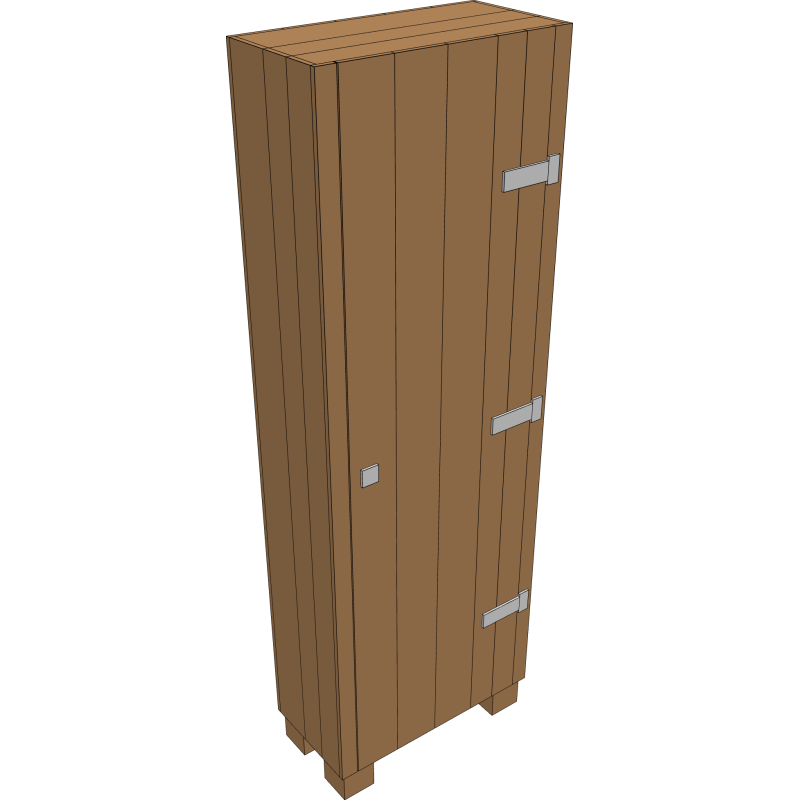
\includegraphics[width=\textwidth]{scene 12 - compleet.png}
\end{figure}

\clearpage
\newpage

\tableofcontents

\clearpage
\newpage

\section{Introductie}

Hartelijk dank voor uw vertrouwen in deze handleiding. In dit document staat stapsgewijs beschreven hoe u de door u opgegeven kast in elkaar kunt zetten. Dit hoofdstuk licht kort de verschillende onderdelen van het assemblageproces toe. In hoofdstuk twee wordt de boodschappenlijst besproken. Het derde hoofdstuk richt zich op de assemblage van uw nieuwe kast. Alle maten in die in deze handleiding zijn beschreven zijn in centimeters tenzij anders aangegeven. \\

Ondanks dat er met enorm veel aandacht aan dit model is gewerkt kan het altijd voorkomen dat er fouten in het model zitten. Wij raden u dan ook aan dat u voor dat u onderdelen aanschaft aandachtig het document doorleest op fouten of inconsistenties. Mocht u fouten tegen komen, zou u dat aan ons kunnen laten weten ? Dan passen wij de fout aan en krijgt u zowel uw geld terug voor deze handleiding als de aangepaste assemblage handleiding. Wij zijn \underline{niet} verantwoordelijk voor eventuele schade (zowel fysiek als financieel) als gevolg van het volgen van deze handleiding. \\

De door ontworpen kast heeft de volgende buiten afmetingen en verdiepingen: \\

\begin{table}[h!]
\centering
\caption{Basis afmetingen kast}
\begin{tabular}{rrr}
\toprule
 breedte &  hoogte &  diepte \\
\midrule
     300 &     300 &      50 \\
\bottomrule
\end{tabular}
\end{table}
 

\begin{center}
\textbf{Heel veel plezier gewenst met deze assemblage en uw nieuwe kast!}
\end{center}

\begin{figure}[h!]
    \centering
    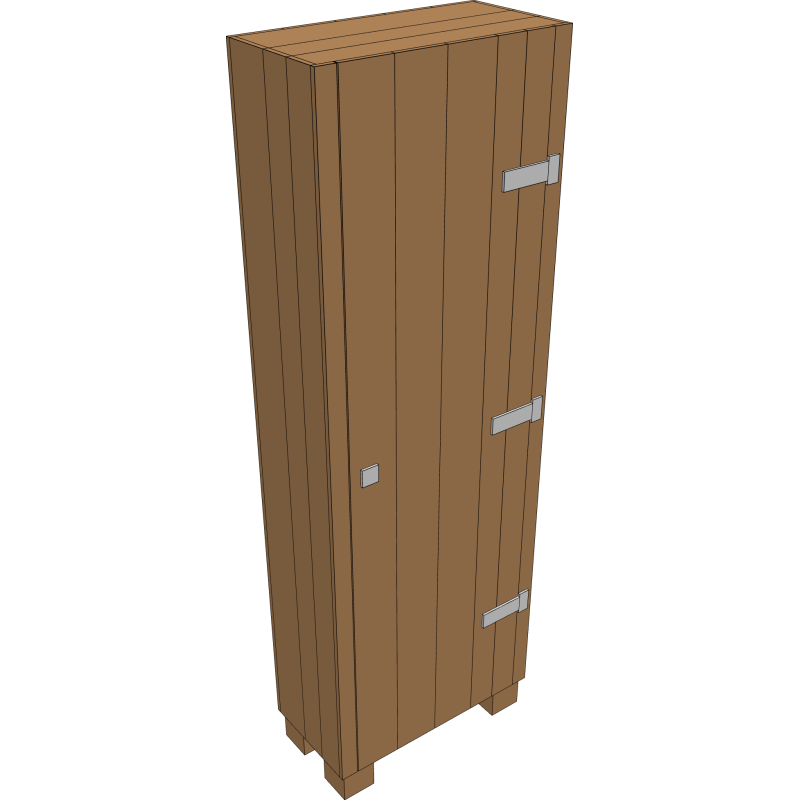
\includegraphics[width=0.7\textwidth]{scene 12 - compleet.png}
\end{figure}

\clearpage
\newpage

\section{Boodschappenlijst}

Om de kast te kunnen assembleren heeft u de volgende materialen en gereedschappen nodig. \\

\subsection{Materialen}

Allereerst de planken en balken. Hiervoor kunt u zowel geschaafd als niet geschaafd hout gebruiken. Niet geschaafd hout is goedkoper, maar let op dat de afmetingen van deze planken en balken kan afwijken.  Het is daardoor wellicht nodig om tijdens de constructie af en extra hout te verwijderen als gevolg van de afwijkende maten.

\begin{table}[h!]
\centering
\caption{Required planks and beams for construction}
\begin{tabular}{lrrrr}
\toprule
 type &  width &  thickness &  length &  ammount \\
\midrule
plank &     20 &          2 &     300 &       23 \\
 beam &      3 &          3 &     300 &        6 \\
\bottomrule
\end{tabular}
\end{table}


Voor de poten zijn de volgende eigenschappen opgesteld. U bent hier vrij iedere vorm poten te kiezen zolang het aantal en de hoogte van de gekozen poten overeen komt met de tabel hier onder.

\begin{table}[h!]
\centering
\caption{Eigenschappen van kastpoten}
\begin{tabular}{rr}
\toprule
 aantal poten &  hoogte \\
\midrule
            8,0 &     5,0 \\
\bottomrule
\end{tabular}
\end{table}


Hieronder is de tabel van de benodigde schroeven weergegeven. Wij raden u aan om houtschroeven te gebruiken met een M4 diameter. \href{https://www.amazon.nl/gp/product/B00B214ZLQ/ref=ppx_yo_dt_b_asin_title_o07_s00?ie=UTF8&psc=1}{Deze M4 houtschroeven} (figuur \ref{fig:schroeven}) zijn een goede optie. Let op dat de lengte van de schroef afwijkend kan zijn voor uw kast. Selecteer een schroef die een lengte heeft dicht bij de 'max lengte'. Neem geen langere schroeven, deze zullen door het hout gaan wat geen mooie afwerking geeft.

\begin{table}[h!]
\centering
\caption{Benodigde schroeven voor constructie}
\begin{tabular}{lrr}
\toprule
{} &  max lengte &  aantal \\
\midrule
Schroef 1 &           5 &       0 \\
Schroef 2 &           3 &       0 \\
Schroef 3 &           4 &       0 \\
\bottomrule
\end{tabular}
\end{table}


\begin{figure}[h!]
    \centering
    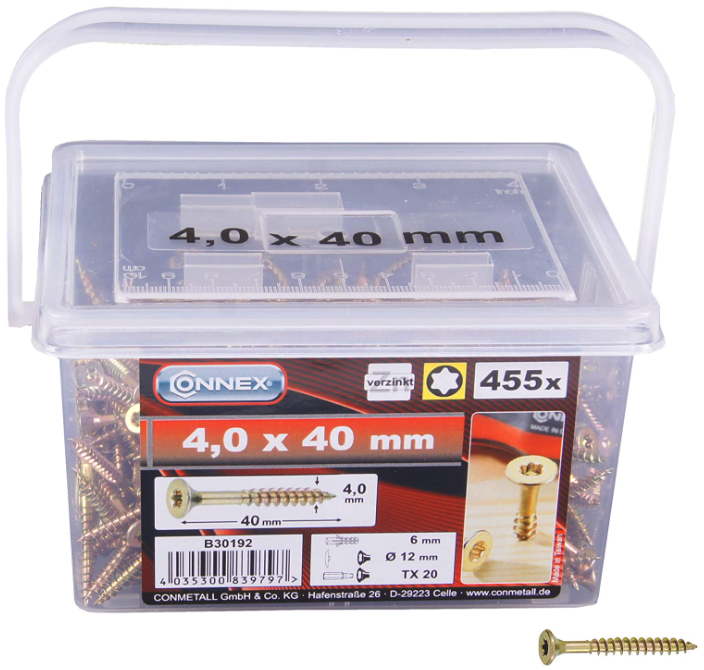
\includegraphics[width=0.3\textwidth]{schroeven.png}
    \caption{Connex M4 Schroeven via Amazon}
    \label{fig:schroeven}
\end{figure}

\clearpage
\newpage

Tot slot zijn er nog extra metalen onderdelen nodig voor de constructie. Voor de hoek frames wordt aangeraden een te selecteren met 4 gaten en een maximale breedte van 3 centimeter. Deze zorgen voor een stevige verbinding. \href{https://www.amazon.nl/Connex-HVG2400-voordeelpak-hoekverbinder-verzinkt/dp/B00J7L2ET8/ref=sr_1_9?__mk_nl_NL=%C3%85M%C3%85%C5%BD%C3%95%C3%91&crid=22ED59WFFPB0Z&keywords=hoekverbinder&qid=1660427081&sprefix=hoekverbinder%2Caps%2C85&sr=8-9}{Deze hoek verbindingen} (figuur \ref{fig:hoeken}) zijn een goede optie. Voor de scharnieren en sloten bent u natuurlijk geheel vrij te kiezen welke het beste bij uw persoonlijke smaak passen.

\begin{table}[h!]
\centering
\caption{Overige benodigde onderdelen voor constructie}
\begin{tabular}{llr}
\toprule
{} & gaten raamwerk &  aantal \\
\midrule
Hoek verbinding &              4 &       0 \\
Scharnier       &         max 10 &       0 \\
Slot            &          max 4 &       0 \\
\bottomrule
\end{tabular}
\end{table}


\begin{figure}[h!]
    \centering
    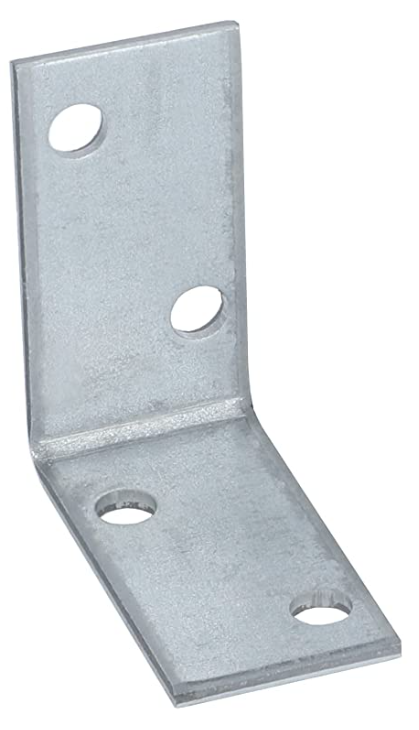
\includegraphics[width=0.2\textwidth]{hoeken.png}
    \caption{Connex hoek verbindingen via Amazon}
    \label{fig:hoeken}
\end{figure}

\subsection{Gereedschappen}

Voor het bouwen van deze kast zijn de onderstaande gereedschappen vereist.

\begin{itemize}
    \item Potlood 
    \item Zaagtafel
    \item Schroefmachine
    \item Rolmaat
\end{itemize}

Daarnaast zijn de volgende onderdelen optioneel. Als u gebruik maakt van hout dat niet geschaafd is zijn onderstaande onderdelen in het bijzonder aangeraden omdat niet-geschaafde planken een aanzienlijke afwijking kunnen hebben in dikte, breedte en rechtheid.

\begin{itemize}
    \item Decoupeerzaag
    \item Schaaf
    \item Blokhaak
\end{itemize}

\begin{center}
    \textit{Tip: heeft u gereedschappen niet bij de hand ? Probeer deze dan eens via \href{https://www.peerby.com/en-nl}{Peerby} te zoeken!}
\end{center}

\clearpage
\newpage

\section{Zaaglijst}

\subsection{Planken en balken lengte}

In de onderstaande tabel is weergegeven hoe de balken en planken \underline{op lengte} worden gezaagd. Er is berekend wat het minimum benodigd aantal planken en balken is, als u deze zaag lijst niet volgt kunt u hout te kort komen.

\begin{table}[h!]
\centering
\caption{Zaaglijst lengte per plank, Totaal 55 planken}
\begin{tabular}{lrrrr}
\toprule
{} &     1 &    2 &    3 &  aantal \\
\midrule
1 &  90,0 & 90,0 & 90,0 &       3 \\
2 & 295,0 &  0,0 &  0,0 &      40 \\
3 & 296,0 &  0,0 &  0,0 &      12 \\
\bottomrule
\end{tabular}
\end{table}


\begin{table}[h!]
\centering
\caption{Sawlist length per beam, Totalling to 6 beams}
\begin{tabular}{lrrrrrr}
\toprule
{} &     1 &    2 &    3 &    4 &    5 &  ammount \\
\midrule
1 &  40,0 & 40,0 & 40,0 & 40,0 & 40,0 &        1 \\
2 &  90,0 & 90,0 & 40,0 & 40,0 & 40,0 &        1 \\
3 & 281,0 &  0,0 &  0,0 &  0,0 &  0,0 &        4 \\
\bottomrule
\end{tabular}
\end{table}


\subsection{Planken en balken breedte}

Nu de planken en balken gezaagd zijn moeten een aantal van de planken ook in de breedte van lengte worden aangepast. Selecteer de planken uit de lijst en zaag ze op de benodigde breedte. \\

\begin{center}
    \textit{Tip: schrijf met een potlood de afmetingen op de planken en balken om ze later snel te kunnen vinden!}
\end{center}

\begin{table}[h!]
\centering
\caption{Partlist beams and planks}
\begin{tabular}{lrrrr}
\toprule
 type &  width &  thickness &  length &  ammount \\
\midrule
 beam &    3,0 &        3,0 &    40,0 &        8 \\
 beam &    3,0 &        3,0 &    90,0 &        2 \\
 beam &    3,0 &        3,0 &   281,0 &        4 \\
plank &    7,5 &        2,0 &   285,0 &        2 \\
plank &   12,2 &        2,0 &   285,0 &        2 \\
plank &   13,0 &        2,0 &    96,0 &        4 \\
plank &   13,0 &        2,0 &   285,0 &        4 \\
plank &   20,0 &        2,0 &    85,0 &        3 \\
plank &   20,0 &        2,0 &    96,0 &        6 \\
plank &   20,0 &        2,0 &   285,0 &       10 \\
\bottomrule
\end{tabular}
\end{table}


\clearpage
\newpage

\section{Assemblage}

\subsection{Stap 1 - Bodem en poten}

Allereerst construeert u het onderstel van de kast. In onderstaande tabel zijn de benodigde materialen voor deze stap weergegeven. In deze tabel is de eerste rij de kast poten en de volgende de planken voor de bodem.

\begin{table}[h!]
\centering
\caption{Stap 1 Samenstelling voeten en bodem}
\begin{tabular}{rrrr}
\toprule
 lengte &  breedte &  dikte &  aantal \\
\midrule
    5,0 &      5,0 &    5,0 &       8 \\
  396,0 &      8,0 &    2,0 &       2 \\
  396,0 &     10,0 &    2,0 &       1 \\
\bottomrule
\end{tabular}
\end{table}


In onderstaande afbeelding is weergegeven hoe de poten op de planken worden bevestigd. De volgorde van het leggen van de planken is niet relevant. Voor het vastmaken van de poten in de planken gebruikt u \textbf{tw\'{e}\'{e} schroeven} per poot. Hier voor gebruikt u \textbf{schroef 1} als aangegeven in tabel 4 van hoofdstuk 2.

Weergegeven maten zijn vanaf de linkerkant van de kast tot het begin van de poot. Poten worden aan de uiteinden van de kast geplaatst in de breedte. Onderstaande afbeelding is extra groot in de appendix weergegeven.

\begin{figure}[h!]
    \centering
    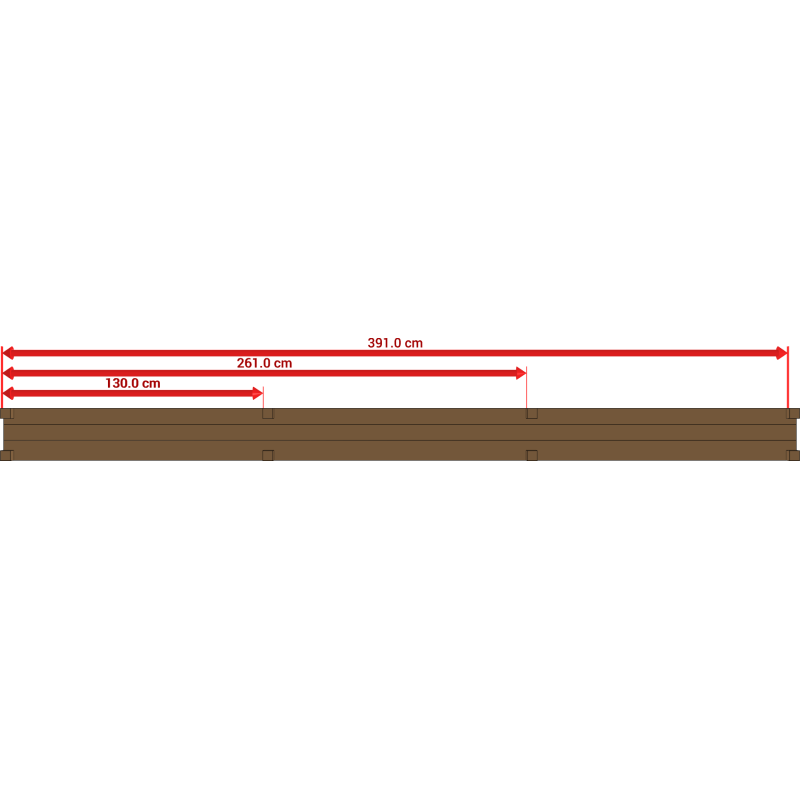
\includegraphics[width=0.8\textwidth]{scene 1 - bottom.png}
    \caption{Onderaanzicht kast}
    \label{fig:stap 1}
\end{figure}

\clearpage
\newpage

\subsection{Stap 2 - Bodem en ribben}

Vervolgens schroeft u de ribben op de kast. In onderstaande tabel zijn de benodigde materialen voor deze stap weergegeven.

\begin{table}[h!]
\centering
\caption{Step 2 Assembly step 1 and bottom rib}
\begin{tabular}{rrrr}
\toprule
 length &  width &  thickness &  ammount \\
\midrule
   40,0 &    3,0 &        3,0 &        2 \\
\bottomrule
\end{tabular}
\end{table}


In onderstaande afbeelding is weergegeven hoe de ribben op de planken worden bevestigd. Voor het vastmaken van de ribben in de planken gebruikt u \textbf{\'{e}\'{e}n schroef per plank per rib}. Hier voor gebruikt u \textbf{schroef 1} als aangegeven in tabel 4 van hoofdstuk 2. Deze schroef gaat eerst door de plank om vervolgens in de balk te eindigen.

Weergegeven maten zijn vanaf de linkerkant van de kast tot het begin van de ribben. De afgebeelde verticaal afstand zorgt er voor dat de ribben in het midden van de planken worden geplaatst. Onderstaande afbeelding is extra groot in de appendix weergegeven.

\begin{figure}[h!]
    \centering
    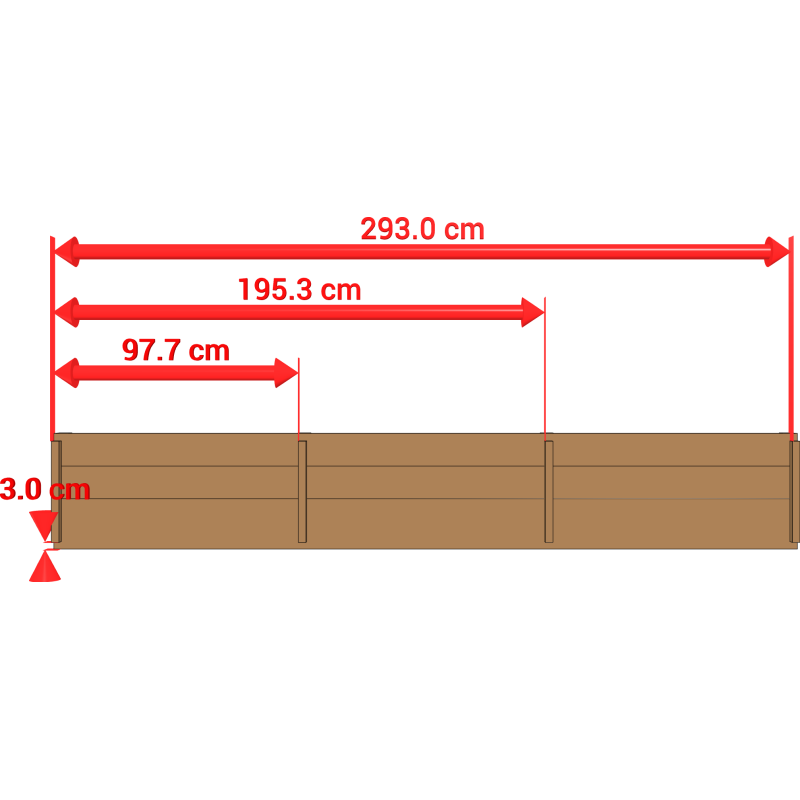
\includegraphics[width=0.8\textwidth]{scene 2 - bottom rib.png}
    \caption{Ribben op kast}
    \label{fig:stap 2}
\end{figure}

\clearpage
\newpage

\subsection{Stap 3 - Ladder frame}

Vervolgens construeert u het het ladder frame. In onderstaande tabel zijn de benodigde materialen voor deze stap weergegeven. Met deze lijst maakt u alle ladder frames voor uw kast, maak hiervoor een gelijke verdeling van de balken voor ieder ladder frame in uw kast.

\begin{table}[h!]
\centering
\caption{Step 3 Ladder frame}
\begin{tabular}{rrrr}
\toprule
 length &  width &  thickness &  ammount \\
\midrule
   40,0 &    3,0 &        3,0 &       16 \\
   94,7 &    3,0 &        3,0 &        9 \\
  291,0 &    3,0 &        3,0 &        8 \\
\bottomrule
\end{tabular}
\end{table}


In onderstaande afbeelding is weergegeven hoe de verticale ribben aan de horizontale balken worden bevestigd. Voor het vastmaken van de ribben in de balken gebruikt u per hoek een hoek verbinding met \textbf{vier schroeven} per verbinding en plaatst u deze op de locatie van de groene pijl. Hier voor gebruikt u \textbf{schroef 2} als aangegeven in tabel 4 van hoofdstuk 2.

Weergegeven maten zijn vanaf de bovenkant van het frame tot het begin van de rib geplaatst. Onderstaande afbeelding is extra groot in de appendix weergegeven.

\begin{figure}[h!]
    \centering
    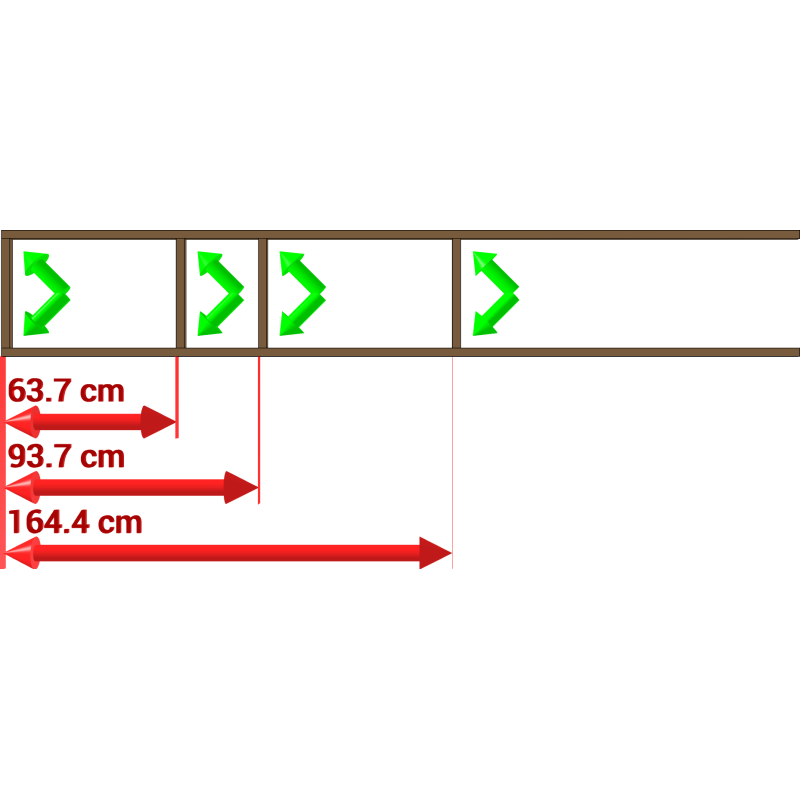
\includegraphics[width=0.8\textwidth]{scene 3 - ladder.png}
    \caption{Ladder frame}
    \label{fig:stap 3}
\end{figure}

\clearpage
\newpage

\subsection{Stap 4 - Ladder op onderstel}

Vervolgens verbindt u de ladder met het onderstel van de kast.

In onderstaande afbeelding is weergegeven hoe de ladder op het onderstel wordt bevestigd. Voor het vastmaken van de ladder aan de ribben gebruikt u per hoek een hoek verbinding met \textbf{vier schroeven} per verbinding en plaatst u deze op de locatie van de groene pijl. Hier voor gebruikt u \textbf{schroef 2} als aangegeven in tabel 4 van hoofdstuk 2.
Onderstaande afbeelding is extra groot in de appendix weergegeven.

\begin{center}
\textit{Let op dat in deze stap de constructie instabiel kan zijn, let dus op dat de ladders niet omvallen! Door gebruik van goede hoek verbindingen zorgt u ervoor dat de constructie in deze stap stabiel blijft.}
\end{center}

\begin{figure}[h!]
    \centering
    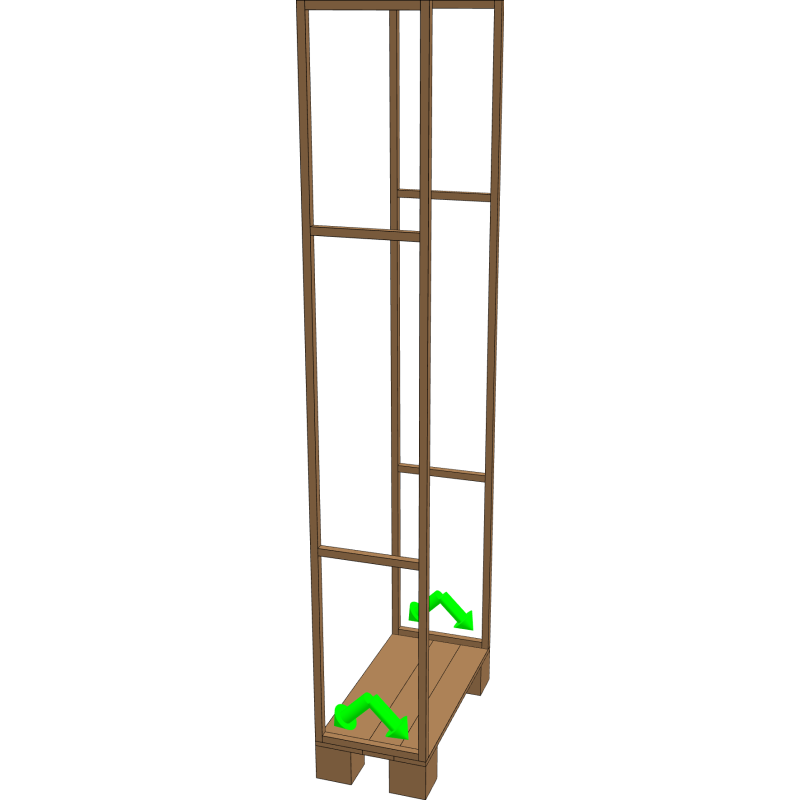
\includegraphics[width=0.8\textwidth]{scene 4 - geraamte.png}
    \caption{Ladders op onderstel}
    \label{fig:stap 4}
\end{figure}

\clearpage
\newpage

\subsection{Stap 5 - Achter ribben}

Vervolgens construeert u achter ribben stelsel van de kast. In onderstaande tabel zijn de benodigde materialen voor deze stap weergegeven.

\begin{table}[h!]
\centering
\caption{Stap 5 Samenstelling stap 2, stap 3 en achter rib}
\begin{tabular}{rrrr}
\toprule
 lengte &  breedte &  dikte &  aantal \\
\midrule
  128,0 &      3,0 &    3,0 &       3 \\
\bottomrule
\end{tabular}
\end{table}


In onderstaande afbeelding is weergegeven hoe de ribben worden verbonden met de achter ribben. Voor het vastmaken van de ribben aan de achter rib gebruikt u per hoek een hoek verbinding met \textbf{vier schroeven} per verbinding en plaatst u deze op de locatie van de groene pijl. Hier voor gebruikt u \textbf{schroef 2} als aangegeven in tabel 4 van hoofdstuk 2.

Weergegeven maten zijn vanaf de bovenkant van de horizontale ribben in de ladder tot de bovenkant van de achter rib. De grootte van de afstand is gelijk aan de dikte van de plank in de verdieping. Onderstaande afbeeldingen zijn extra groot in de appendix weergegeven.

\begin{figure}[h!]
    \centering
    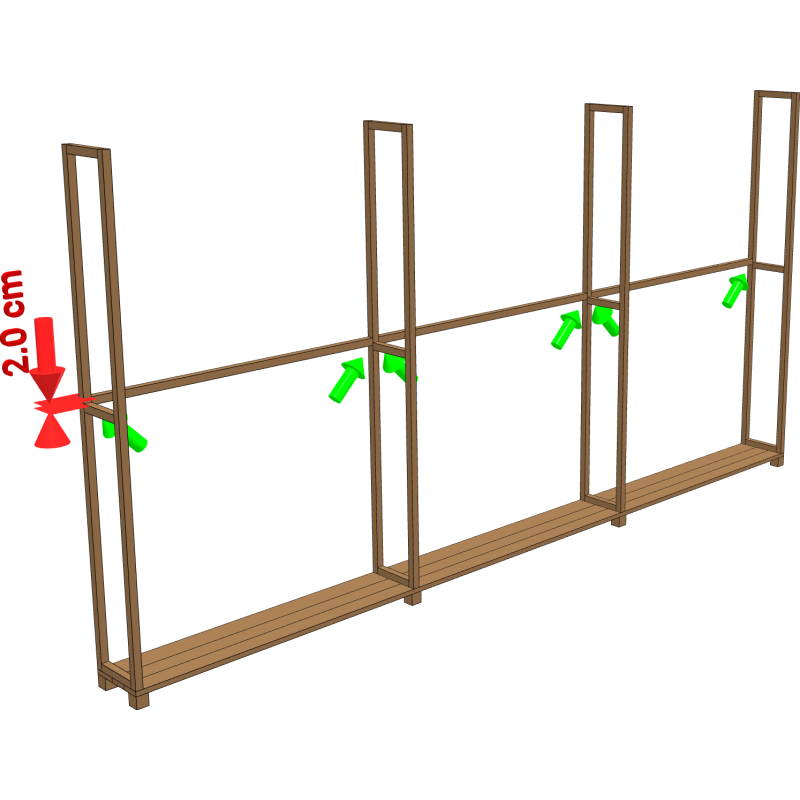
\includegraphics[width=0.8\textwidth]{scene 5 - achterrib a.png}
    \caption{Achter rib globaal}
    \label{fig:stap 5a}
\end{figure}

\begin{figure}[h!]
    \centering
    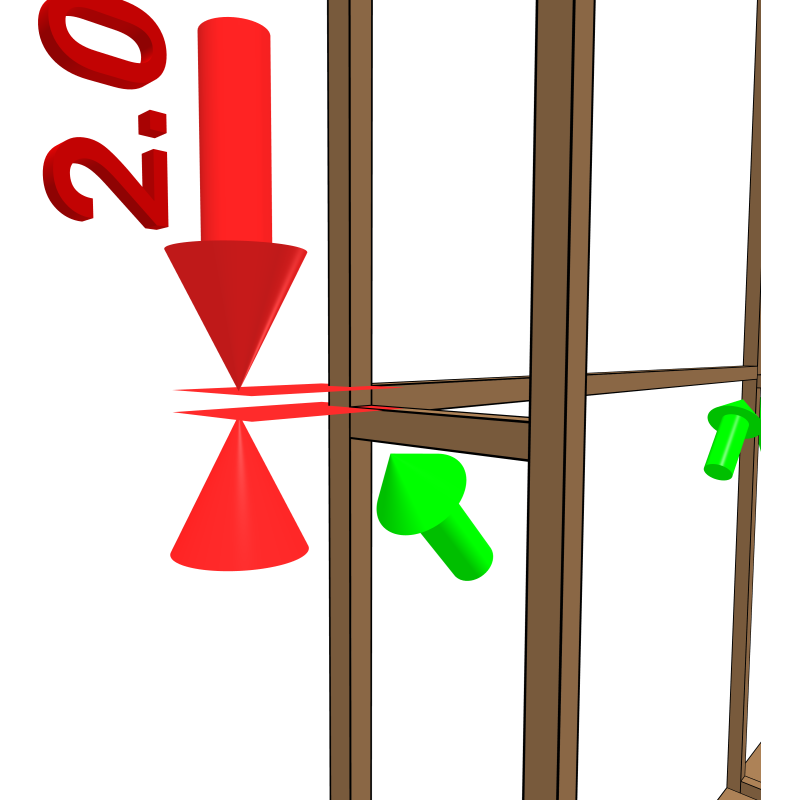
\includegraphics[width=0.8\textwidth]{scene 5 - achterrib b.png}
    \caption{Achter rib lokaal}
    \label{fig:stap 5b}
\end{figure}

\clearpage
\newpage

\subsection{Stap 6 - Vlonders}

Nu is het tijd om de vlonders van uw kast te plaatsen. In onderstaande tabel zijn de benodigde materialen voor deze stap weergegeven. Met deze lijst maakt u alle vlonders voor uw kast, maak hiervoor een gelijke verdeling van de planken voor iedere verdieping in uw kast.

\begin{table}[h!]
\centering
\caption{Step 6 Assembly step 5 and platforms}
\begin{tabular}{rrrr}
\toprule
 length &  width &  thickness &  ammount \\
\midrule
   96,0 &   20,0 &        2,0 &        4 \\
\bottomrule
\end{tabular}
\end{table}


In onderstaande afbeelding is weergegeven hoe de planken worden verbonden met de ribben van de ladder. De volgorde van het leggen van de planken is niet relevant. Om de planken aan de ribben te bevestigen schroeft u iedere plank \textbf{met \'{e}\'{en} schroef} vast voor iedere locatie waar deze in contact komt met een rib van de ladder. Hiervoor gebruikt u \textbf{schroef 1} als aangegeven in tabel 4 van hoofdstuk 2. Deze schroef gaat eerst door de plank om vervolgens in de balk te eindigen.

Weergegeven maten zijn vanaf de bovenkant van de horizontale ribben in de ladder tot de bovenkant van de achter rib. Onderstaande afbeeldingen zijn extra groot in de appendix weergegeven.

\begin{figure}[h!]
    \centering
    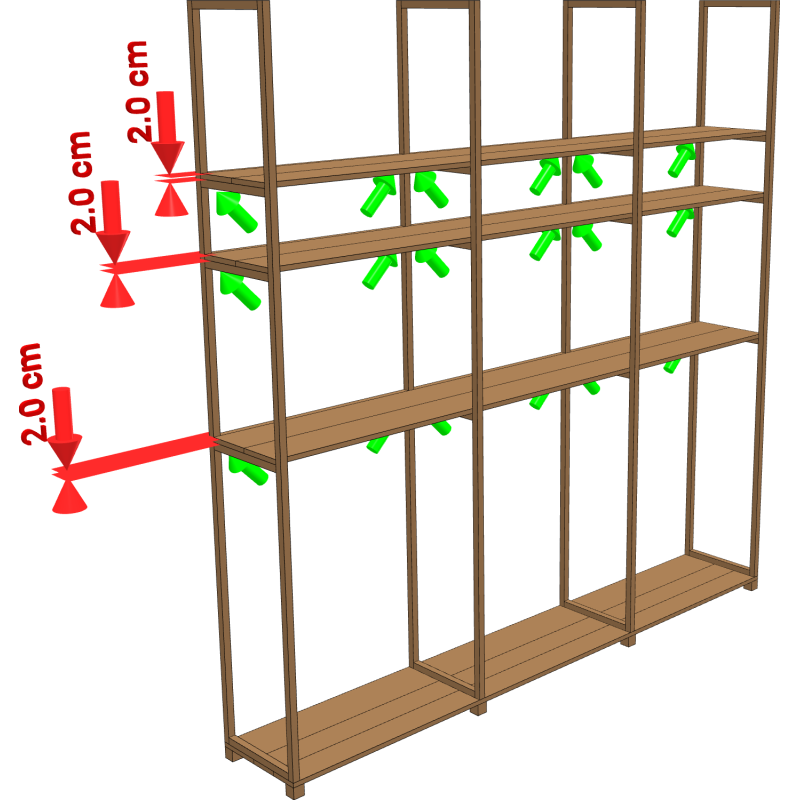
\includegraphics[width=0.8\textwidth]{scene 6 - vlonders a.png}
    \caption{Vlonders globaal}
    \label{fig:stap 6a}
\end{figure}

\begin{figure}[h!]
    \centering
    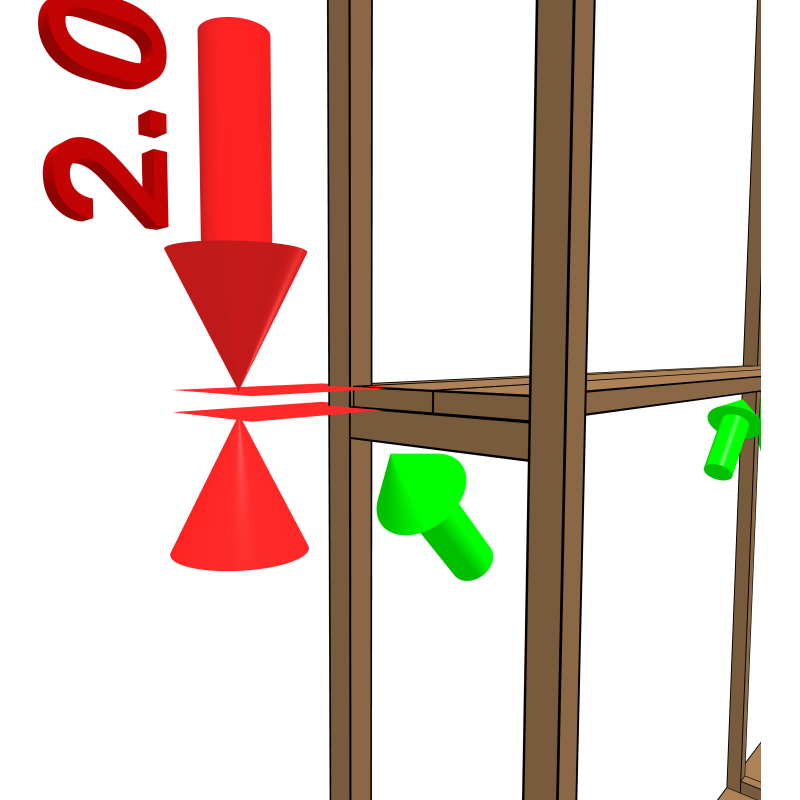
\includegraphics[width=0.8\textwidth]{scene 6 - vlonders b.png}
    \caption{Vlonders lokaal}
    \label{fig:stap 6b}
\end{figure}

\clearpage
\newpage

\subsection{Stap 7 - Bovenkant}

Nu is het tijd om de omkapping van de kast te bouwen. In onderstaande tabel zijn de benodigde materialen voor deze stap weergegeven.

\begin{table}[h!]
\centering
\caption{Stap 7 Samenstelling stap 6 en bovenkant}
\begin{tabular}{rrrr}
\toprule
 lengte &  breedte &  dikte &  aantal \\
\midrule
  296,0 &     13,0 &    2,0 &       2 \\
  296,0 &     20,0 &    2,0 &       1 \\
\bottomrule
\end{tabular}
\end{table}


In onderstaande afbeelding is weergegeven hoe de planken worden verbonden met de ribben van de ladder. Om de planken aan de ribben te bevestigen schroeft u iedere plank \textbf{met \'{e}\'{en} schroef} vast voor iedere locatie waar deze in contact komt met een rib van de ladder. Hiervoor gebruikt u \textbf{schroef 1} als aangegeven in tabel 4 van hoofdstuk 2. Deze schroef gaat eerst door de plank om vervolgens in de balk te eindigen.

Onderstaande afbeeldingen zijn extra groot in de appendix weergegeven.

\begin{figure}[h!]
    \centering
    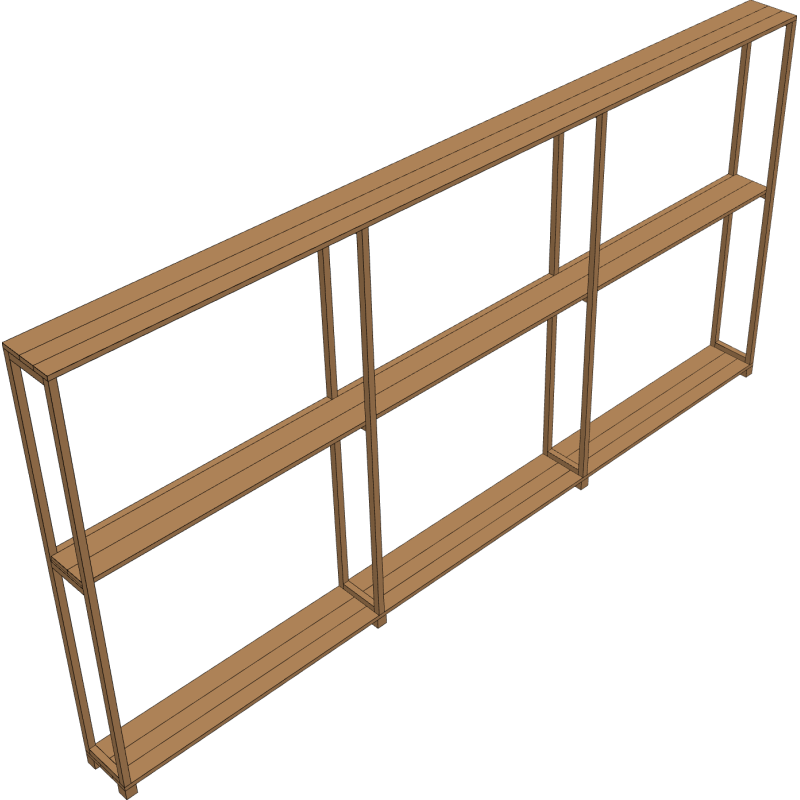
\includegraphics[width=0.8\textwidth]{scene 7 - boven.png}
    \caption{Bovenkant kast}
    \label{fig:stap 7}
\end{figure}

\clearpage
\newpage

\subsection{Stap 8 - Zeiden}

Vervolgens worden de zeiden van de kast geconstrueerd. In onderstaande tabel zijn de benodigde materialen voor deze stap weergegeven. Met deze lijst maakt u alle zeiden voor uw kast, maak hiervoor een gelijke verdeling van de planken voor de linker en rechter zeide.

\begin{table}[h!]
\centering
\caption{Stap 8 Samenstelling stap 7 en zeiden}
\begin{tabular}{rrrr}
\toprule
 lengte &  breedte &  dikte &  aantal \\
\midrule
  195,0 &      8,0 &    2,0 &       4 \\
  195,0 &     10,0 &    2,0 &       2 \\
\bottomrule
\end{tabular}
\end{table}


In onderstaande afbeelding is weergegeven hoe de planken worden verbonden met de horizontale balken van de ladder. De volgorde van het plaatsen van de planken is niet relevant. Om de planken aan de balken te bevestigen schroeft u iedere plank \textbf{met \'{e}\'{en} schroef} vast voor iedere locatie waar deze in contact komt met een horizontale rib van de ladder. Hiervoor gebruikt u \textbf{schroef 1} als aangegeven in tabel 4 van hoofdstuk 2. Deze schroef gaat eerst door de plank om vervolgens in de balk te eindigen. De weergegeven afstanden geven de hoogte aan voor het plaatsen van de schroeven ter hoogte van de ribben. Deze zijn ten opzichte van de onderkant van de kast (onderkant van de poten) weergegeven.

Onderstaande afbeeldingen zijn extra groot in de appendix weergegeven.

\begin{figure}[h!]
    \centering
    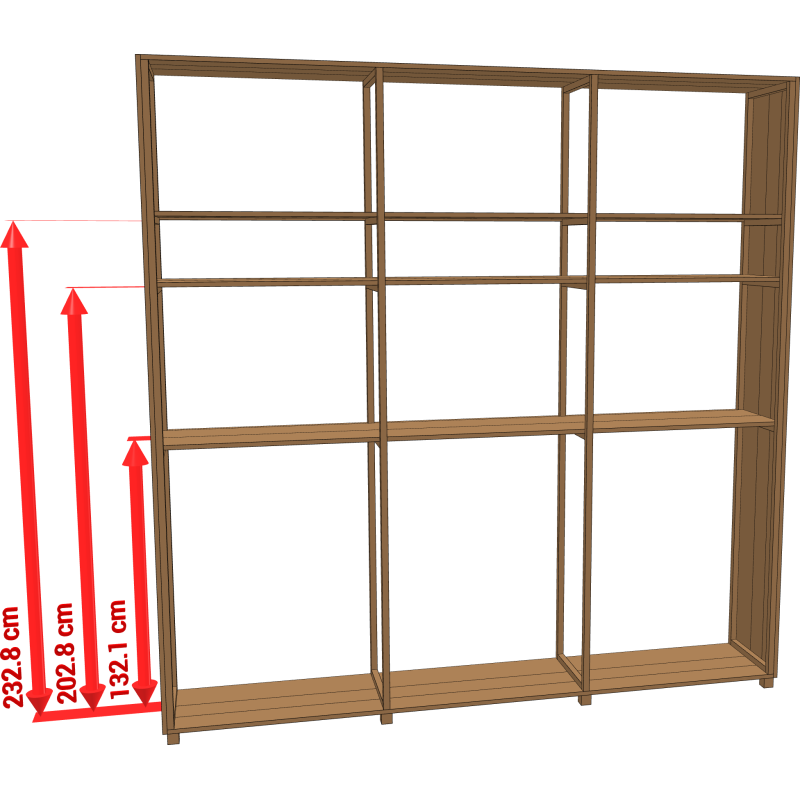
\includegraphics[width=0.8\textwidth]{scene 8 - links_rechts.png}
    \caption{Zeiden kast}
    \label{fig:stap 8}
\end{figure}

\clearpage
\newpage

\subsection{Stap 9 - Achterkant}

Vervolgens wordt de achterkant van de kast geconstrueerd. In onderstaande tabel zijn de benodigde materialen voor deze stap weergegeven.

\begin{table}[h!]
\centering
\caption{Step 9 Assembly step 8 and back side}
\begin{tabular}{rrrr}
\toprule
 length &  width &  thickness &  ammount \\
\midrule
  494,0 &   20,0 &        2,7 &       10 \\
\bottomrule
\end{tabular}
\end{table}


In onderstaande afbeelding is weergegeven hoe de planken worden verbonden met de horizontale achter ribben van de kast. De volgorde van het plaatsen van de planken is niet relevant. Om de planken aan de balken te bevestigen schroeft u iedere plank \textbf{met \'{e}\'{en} schroef} vast voor iedere locatie waar deze in contact komt met een horizontale achter rib van de kast. Hiervoor gebruikt u \textbf{schroef 1} als aangegeven in tabel 4 van hoofdstuk 2. Deze schroef gaat eerst door de plank om vervolgens in de balk te eindigen. De weergegeven afstanden geven de hoogte aan voor het plaatsen van de schroeven ter hoogte van de achter ribben. Deze zijn ten opzichte van de onderkant van de kast (onderkant van de poten) weergegeven.

Onderstaande afbeeldingen zijn extra groot in de appendix weergegeven.

\begin{figure}[h!]
    \centering
    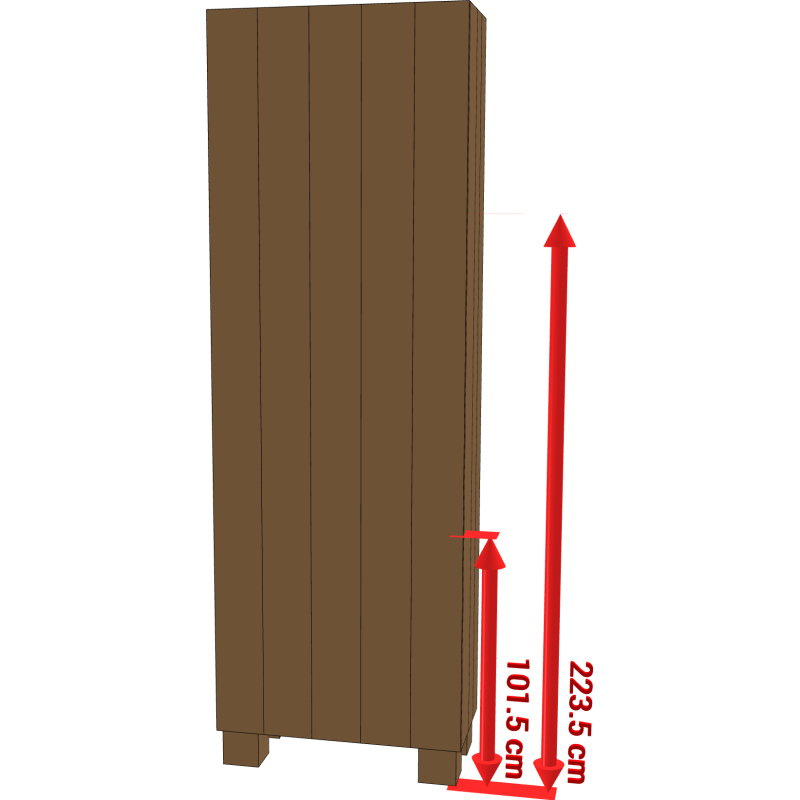
\includegraphics[width=0.8\textwidth]{scene 9 - achterkant.png}
    \caption{Achterkant kast}
    \label{fig:stap 9}
\end{figure}

\clearpage
\newpage

\subsection{Stap 10 - Deurposten}

Nu worden de deurposten van de kast geconstrueerd. In onderstaande tabel zijn de benodigde materialen voor deze stap weergegeven.

\begin{table}[h!]
\centering
\caption{Stap 10 Samenstelling en deurpost(en)}
\begin{tabular}{rrrr}
\toprule
 lengte &  breedte &  dikte &  aantal \\
\midrule
  195,0 &      7,5 &    2,0 &       4 \\
\bottomrule
\end{tabular}
\end{table}


In onderstaande afbeelding is weergegeven hoe de planken worden verbonden aan de voorkant van de kast. Om de planken aan de balken te bevestigen schroeft u iedere plank \textbf{met \'{e}\'{e}n schroef} vast voor iedere locatie ter hoogte van een horizontale rib van de ladder. Hiervoor gebruikt u \textbf{schroef 1} als aangegeven in tabel 4 van hoofdstuk 2. Deze schroef gaat eerst door de plank om vervolgens in de balk te eindigen. De weergegeven afstanden geven de afstand aan van de buitenkant van de kast tot het begin van de plank.

Onderstaande afbeeldingen zijn extra groot in de appendix weergegeven.

\begin{figure}[h!]
    \centering
    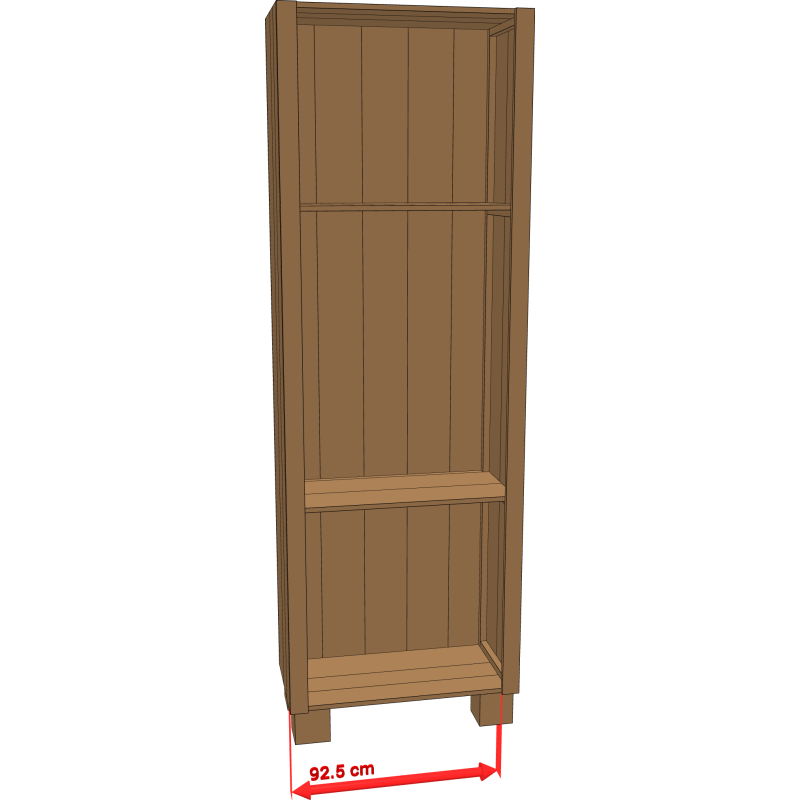
\includegraphics[width=0.8\textwidth]{scene 10 - deurpost a.png}
    \caption{Deurpost globaal}
    \label{fig:stap 10a}
\end{figure}

\begin{figure}[h!]
    \centering
    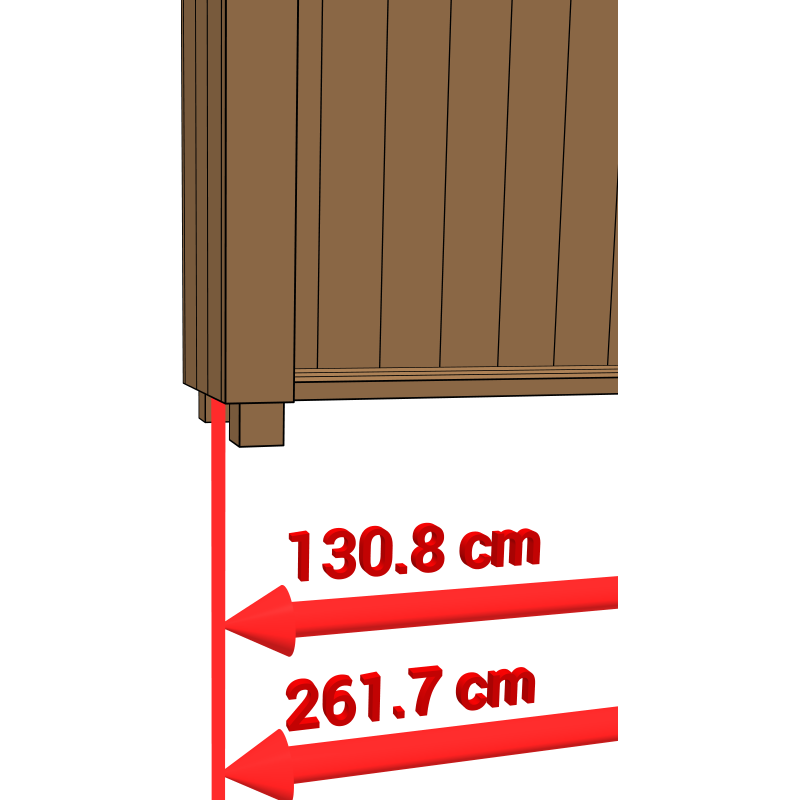
\includegraphics[width=0.8\textwidth]{scene 10 - deurpost b.png}
    \caption{Deurpost lokaal}
    \label{fig:stap 10b}
\end{figure}

\clearpage
\newpage

\subsection{Stap 11 - Deuren}

Vervolgens worden de deuren van de kast geconstrueerd. In onderstaande tabel zijn de benodigde materialen voor deze stap weergegeven. Met deze lijst maakt u \'{e}\'{e}n deur, herhaal deze stap voor het aantal deuren in uw kast.

\begin{table}[h!]
\centering
\caption{Step 11 Door(s)}
\begin{tabular}{rrrr}
\toprule
 length &  width &  thickness &  ammount \\
\midrule
   90,0 &   20,0 &        2,0 &        3 \\
  295,0 &   14,7 &        2,0 &        2 \\
  295,0 &   20,0 &        2,0 &        3 \\
\bottomrule
\end{tabular}
\end{table}


In onderstaande afbeelding is weergegeven op welke hoogte het \textbf{midden} van \textbf{zowel de horizontale planken als de scharnieren} aan de andere kant worden bevestigd. Voor het vastmaken van de planken wordt er \'{e}\'{e}n schroef per horizontale plank per verticale plank gebruikt. Voor ieder scharnier is rekening gehouden met 10 schroeven.  Hier voor gebruikt u \textbf{schroef 3} als aangegeven in tabel 4 van hoofdstuk 2.

De maten zijn gegeven ten opzichte van de onderkant van de deur. Onderstaande afbeelding is extra groot in de appendix weergegeven.

\begin{figure}[h!]
    \centering
    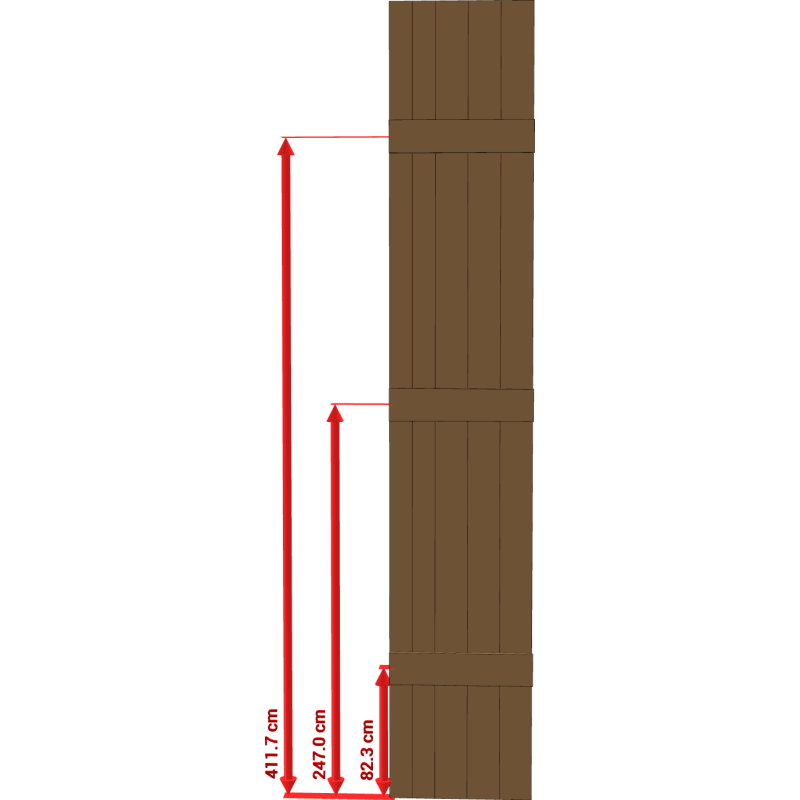
\includegraphics[width=0.8\textwidth]{scene 11 - deur.png}
    \caption{Deur}
    \label{fig:stap 11}
\end{figure}

\clearpage
\newpage

\subsection{Stap 12 - Complete kast}

Tot slot worden de deuren aan de kast bevestigd. Hier kunt u zelf kiezen aan welke zeiden u de scharnieren wilt plaatsen. Zodra de deuren zijn bevestigd kunnen de sloten worden geplaatst. In onderstaande tabel zijn de benodigde materialen voor deze stap weergegeven.

\begin{table}[h!]
\centering
\caption{Stap 12 Scharnieren}
\begin{tabular}{rrrr}
\toprule
 lengte &  breedte &  dikte &  aantal \\
\midrule
    5,0 &     10,0 &    1,0 &       9 \\
   20,0 &      7,0 &    1,0 &       9 \\
\bottomrule
\end{tabular}
\end{table}


In onderstaande afbeelding is een voorbeeld weergegeven hoe de deuren kunnen worden bevestigd aan de kast. Voor het verbinden van de scharnieren en sloten gebruikt u \textbf{schroef 3} als aangegeven in tabel 4 van hoofdstuk 2. Deze schroef gaat eerst door de plank om vervolgens in de balk te eindigen.

Onderstaande afbeeldingen zijn extra groot in de appendix weergegeven.

\begin{figure}[h!]
    \centering
    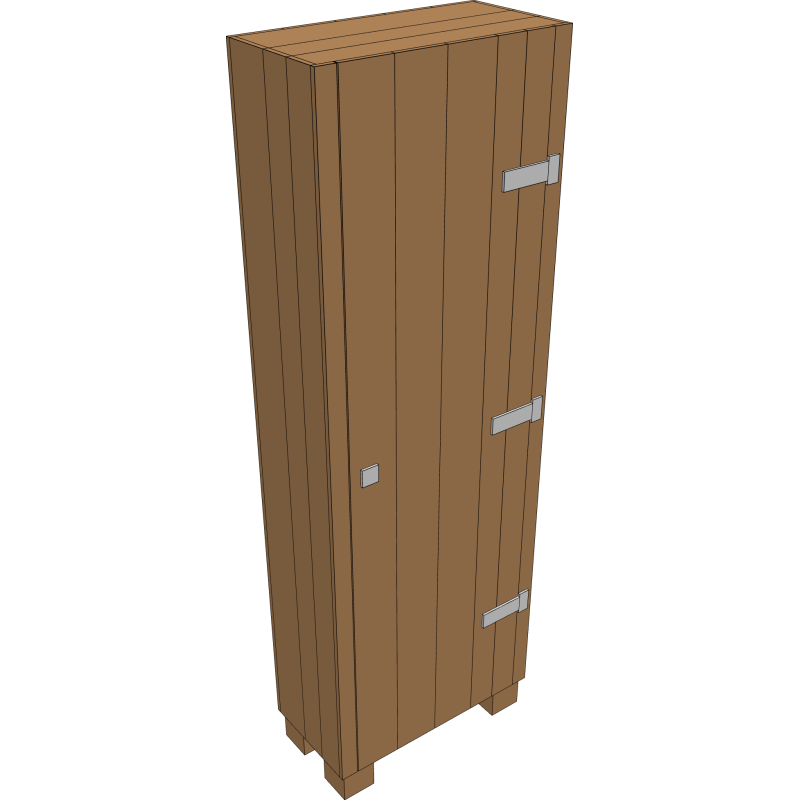
\includegraphics[width=0.8\textwidth]{scene 12 - compleet.png}
    \caption{Uw nieuwe kast is klaar voor gebruik!}
    \label{fig:stap 12}
\end{figure}

\clearpage
\newpage

\section{Appendix}

\begin{figure}[h!]
    \centering
    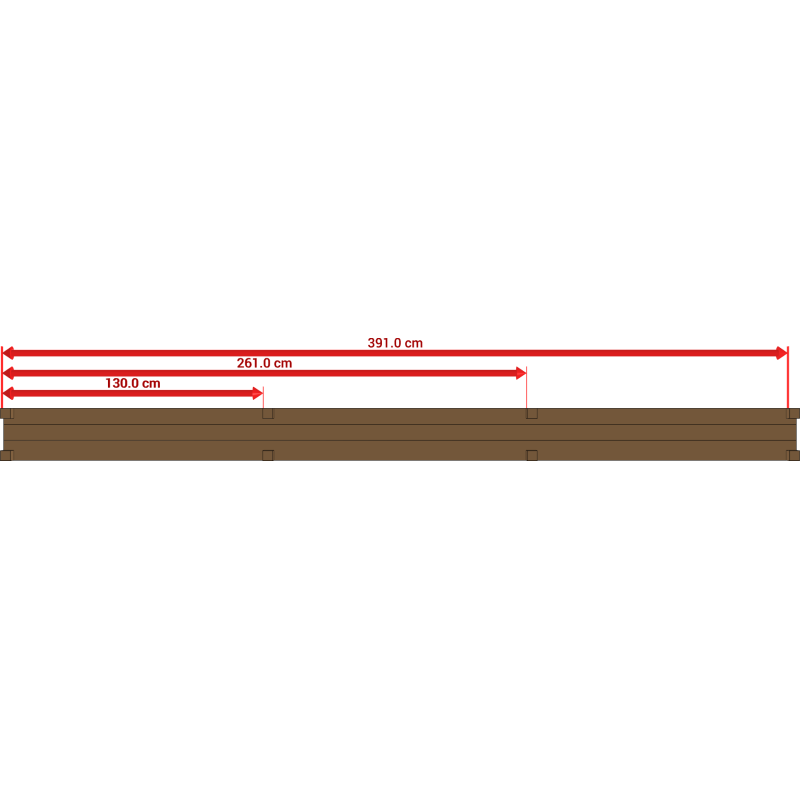
\includegraphics[width=\textwidth]{scene 1 - bottom.png}
    \caption{Onderaanzicht kast}
\end{figure}

\begin{figure}[h!]
    \centering
    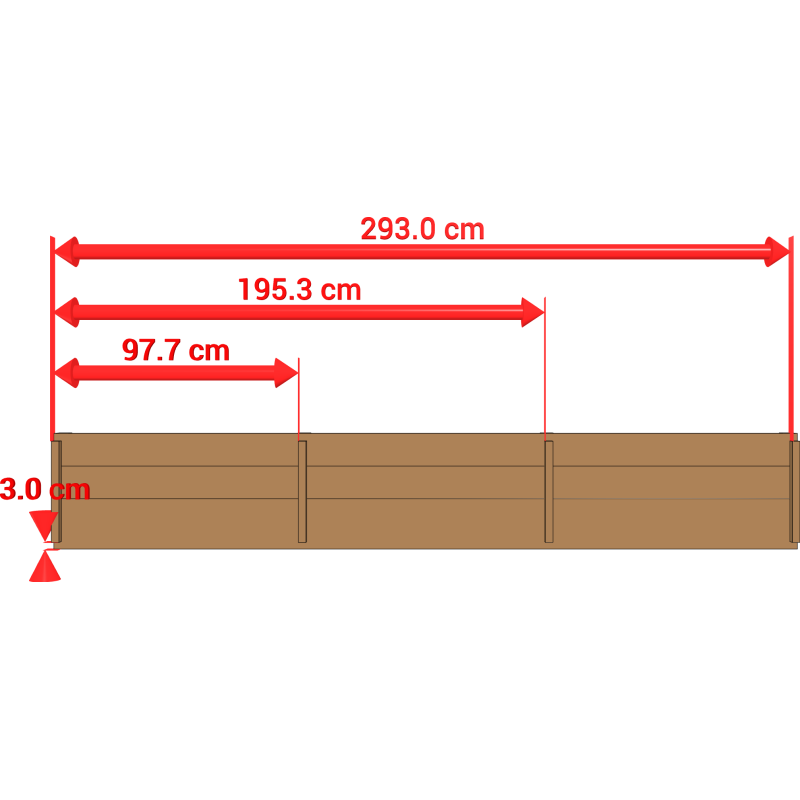
\includegraphics[width=\textwidth]{scene 2 - bottom rib.png}
    \caption{Ribben op kast}
\end{figure}

\begin{figure}[h!]
    \centering
    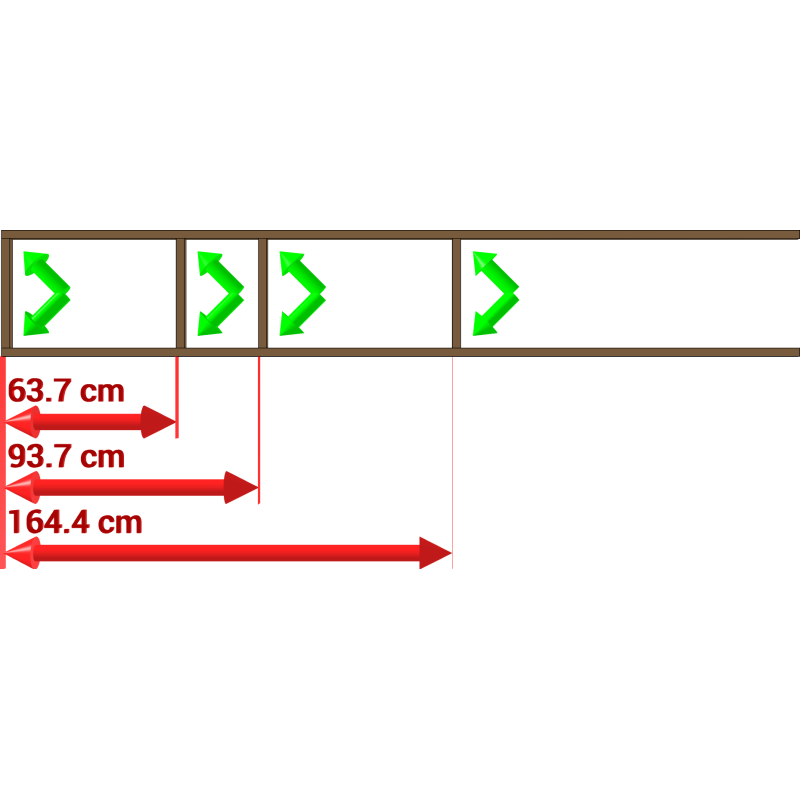
\includegraphics[width=\textwidth]{scene 3 - ladder.png}
    \caption{Ladder frame}
\end{figure}

\begin{figure}[h!]
    \centering
    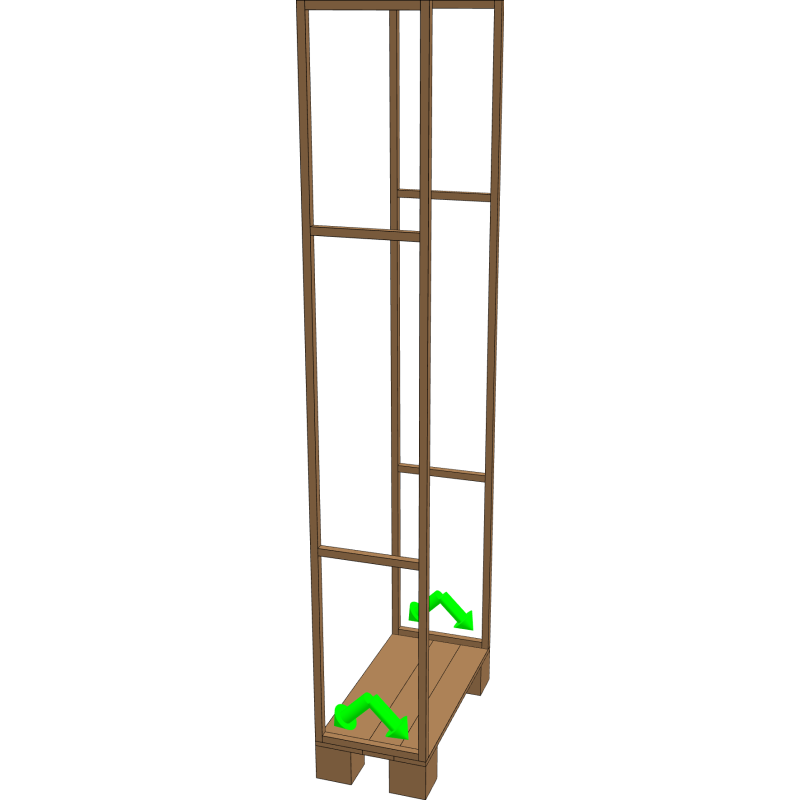
\includegraphics[width=\textwidth]{scene 4 - geraamte.png}
    \caption{Ladders op onderstel}
\end{figure}

\begin{figure}[h!]
    \centering
    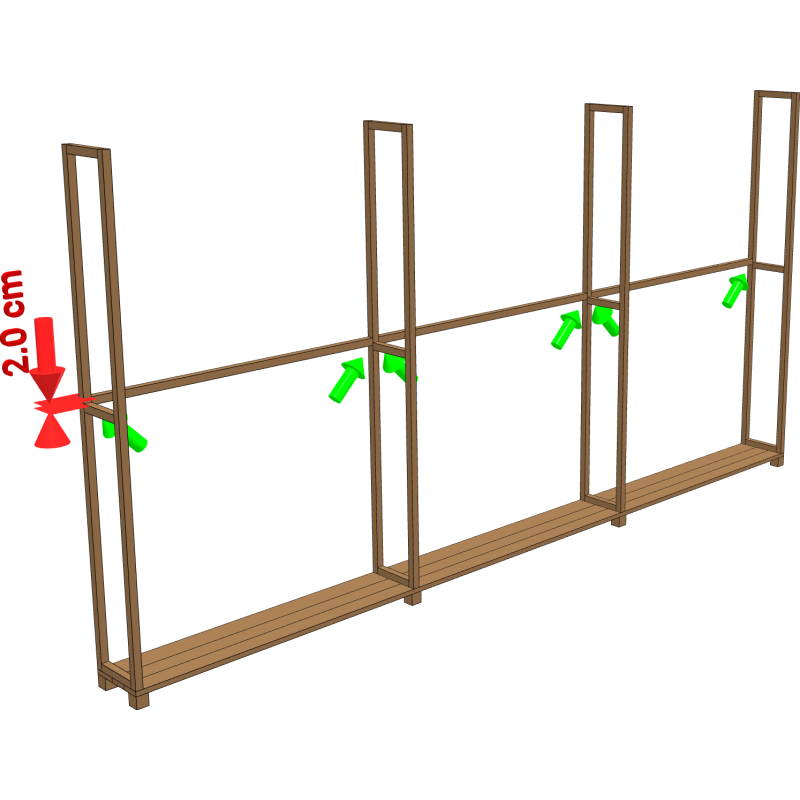
\includegraphics[width=\textwidth]{scene 5 - achterrib a.png}
    \caption{Achter rib globaal}
\end{figure}

\begin{figure}[h!]
    \centering
    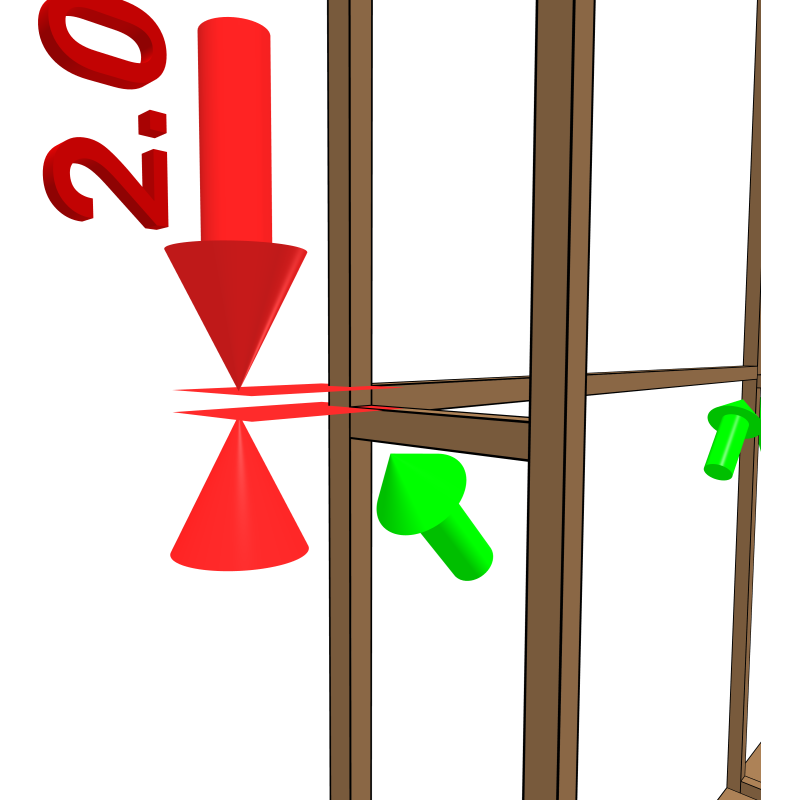
\includegraphics[width=\textwidth]{scene 5 - achterrib b.png}
    \caption{Achter rib lokaal}
\end{figure}

\begin{figure}[h!]
    \centering
    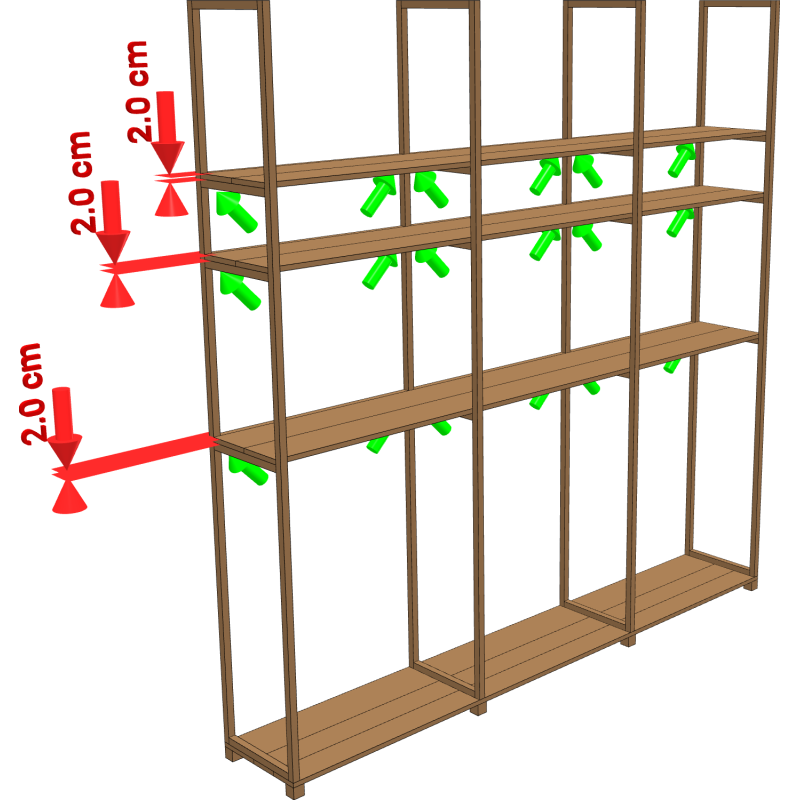
\includegraphics[width=\textwidth]{scene 6 - vlonders a.png}
    \caption{Vlonders globaal}
\end{figure}

\begin{figure}[h!]
    \centering
    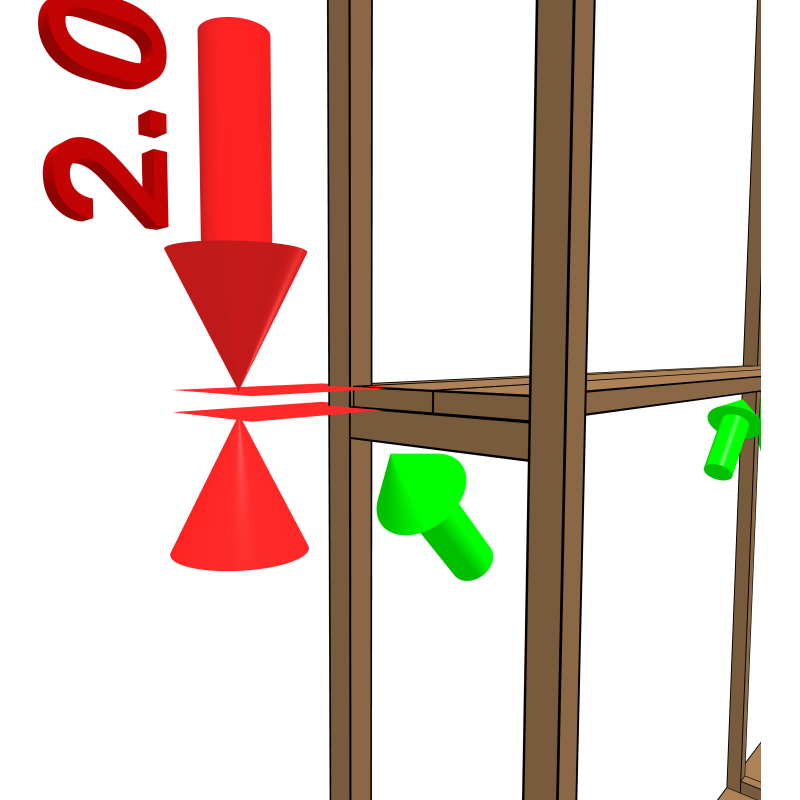
\includegraphics[width=\textwidth]{scene 6 - vlonders b.png}
    \caption{Vlonders lokaal}
\end{figure}

\begin{figure}[h!]
    \centering
    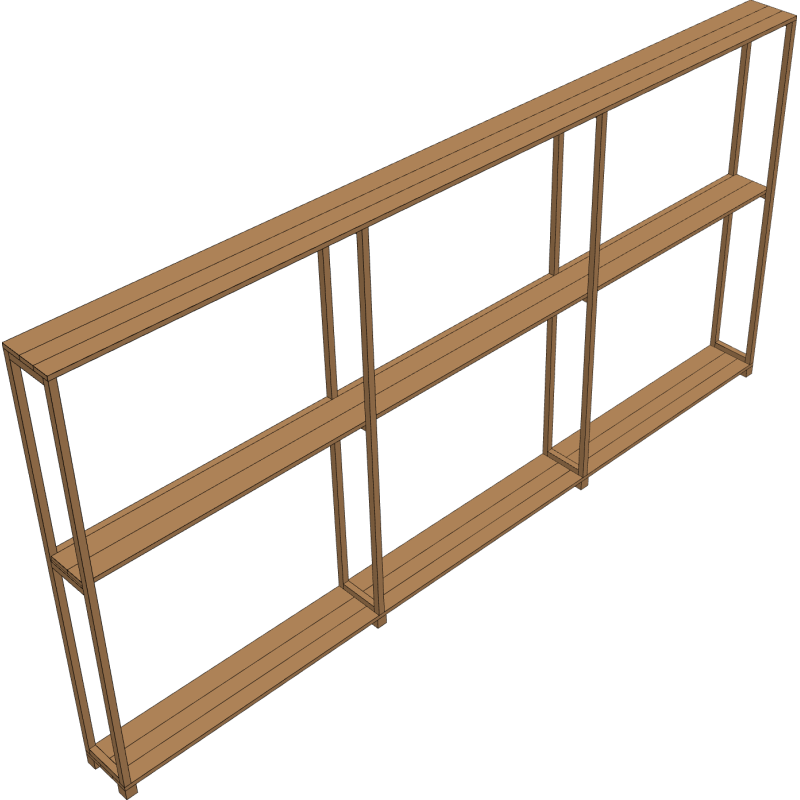
\includegraphics[width=\textwidth]{scene 7 - boven.png}
    \caption{Bovenkant kast}
\end{figure}

\begin{figure}[h!]
    \centering
    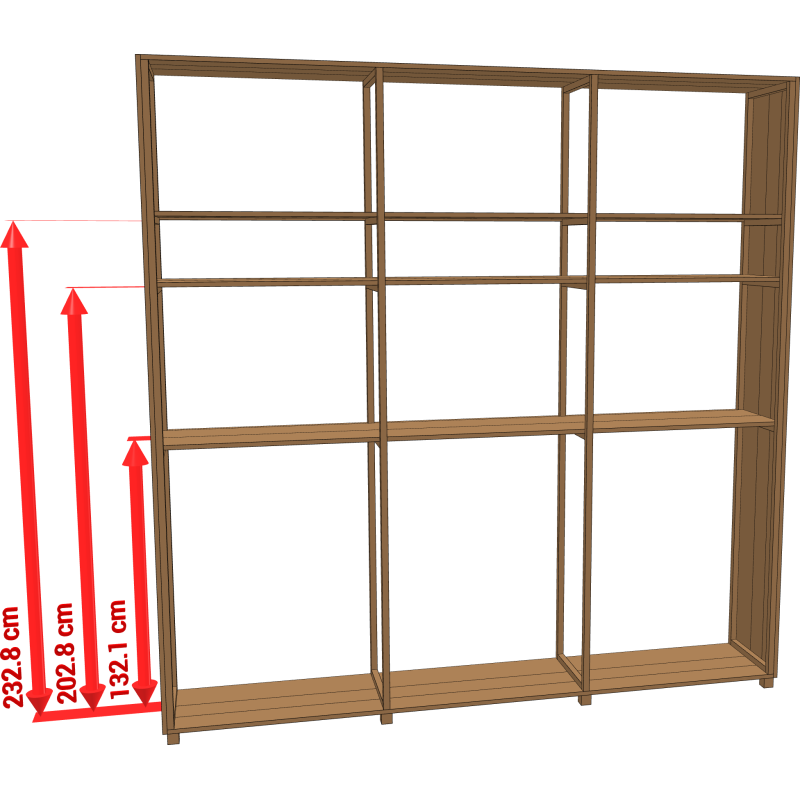
\includegraphics[width=\textwidth]{scene 8 - links_rechts.png}
    \caption{Zeiden kast}
\end{figure}

\begin{figure}[h!]
    \centering
    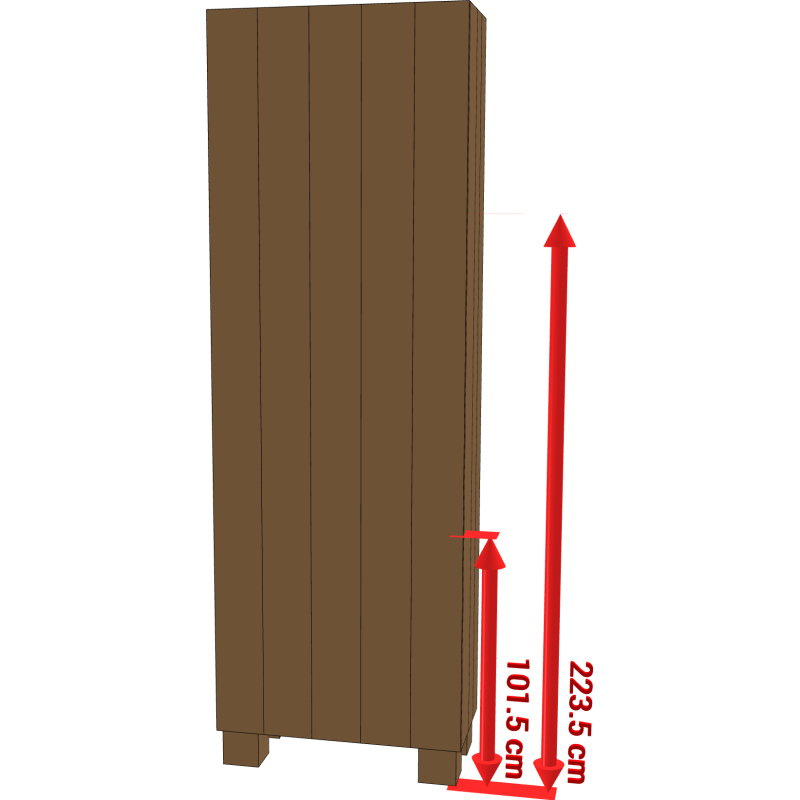
\includegraphics[width=\textwidth]{scene 9 - achterkant.png}
    \caption{Achterkant kast}
\end{figure}

\begin{figure}[h!]
    \centering
    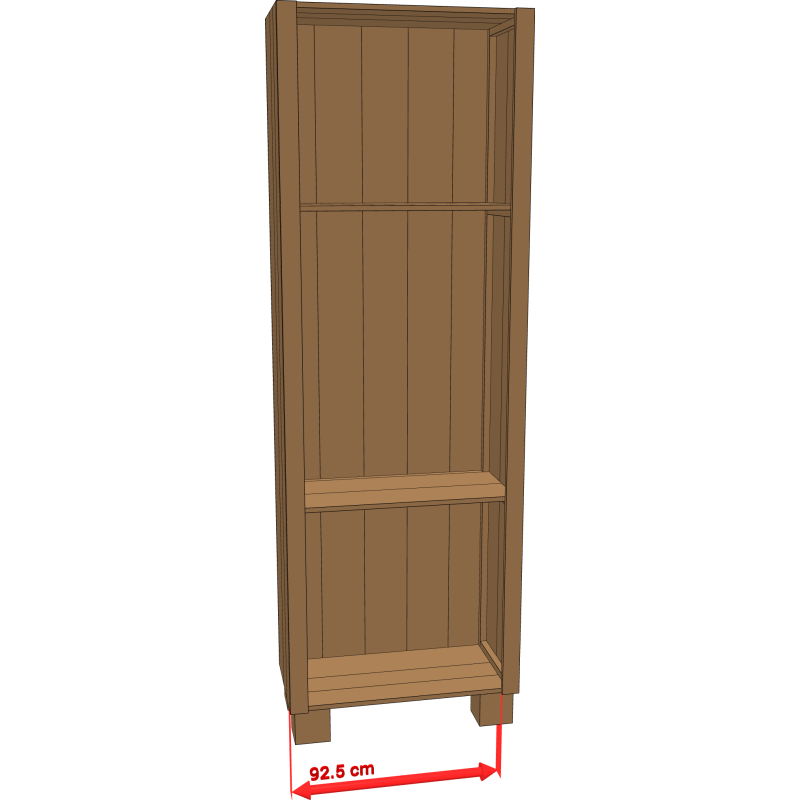
\includegraphics[width=\textwidth]{scene 10 - deurpost a.png}
    \caption{Deurpost globaal}
\end{figure}

\begin{figure}[h!]
    \centering
    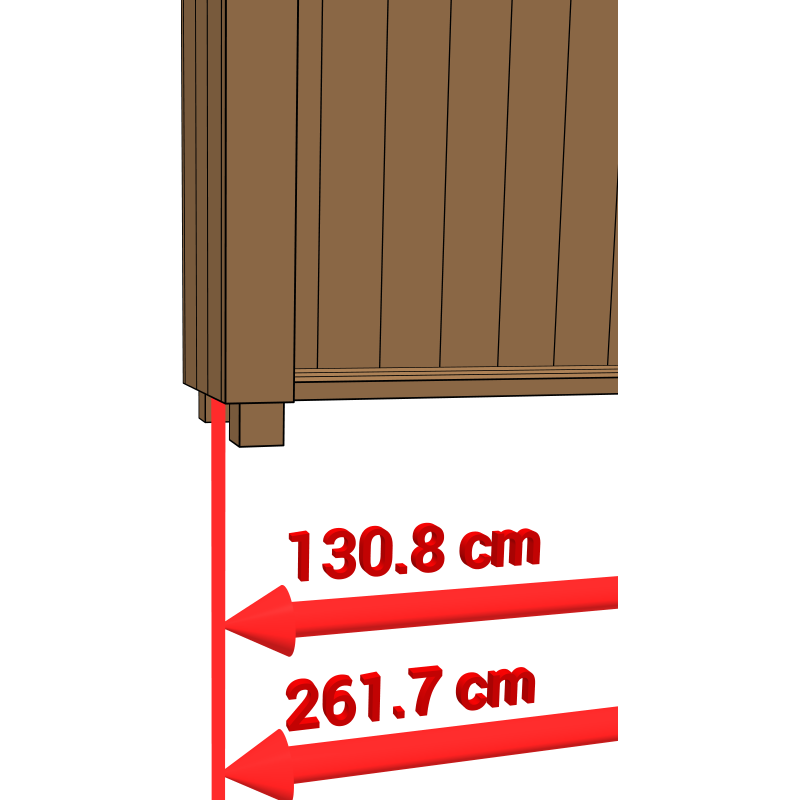
\includegraphics[width=\textwidth]{scene 10 - deurpost b.png}
    \caption{Deurpost lokaal}
\end{figure}

\begin{figure}[h!]
    \centering
    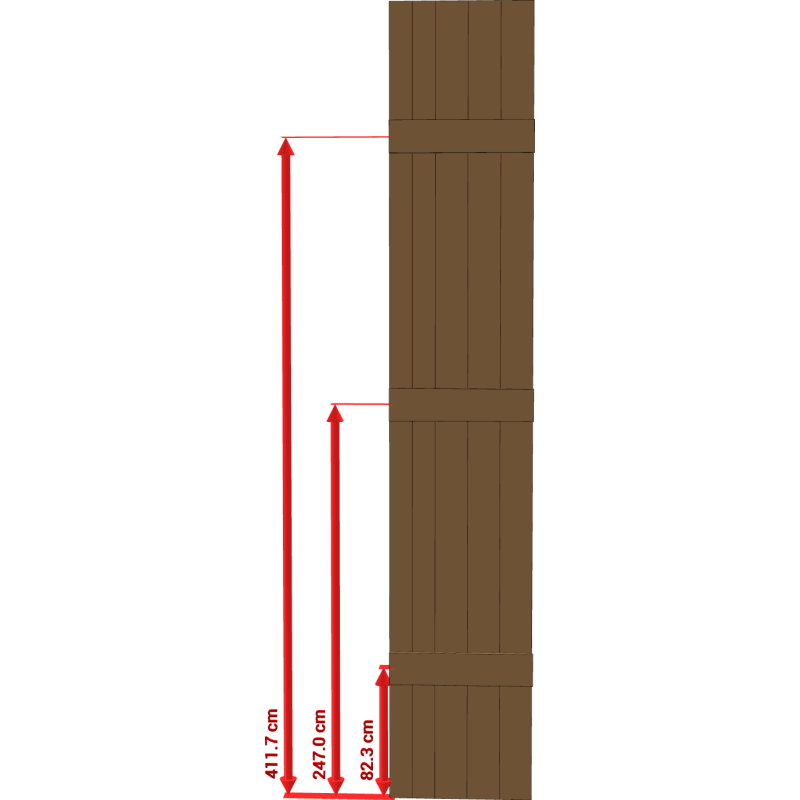
\includegraphics[width=\textwidth]{scene 11 - deur.png}
    \caption{Deur}
\end{figure}

\begin{figure}[h!]
    \centering
    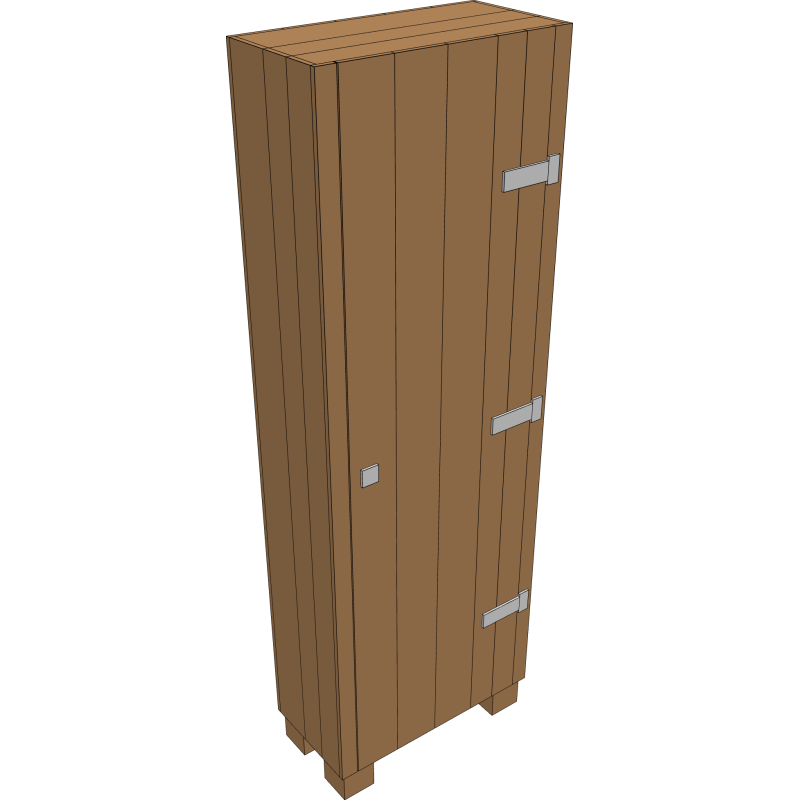
\includegraphics[width=\textwidth]{scene 12 - compleet.png}
    \caption{Uw nieuwe kast is klaar voor gebruik!}
\end{figure}

\end{document}